\documentclass[10pt]{beamer}
\usepackage[utf8]{inputenc}
\usepackage[english]{babel}
\usetheme{Hannover}
\usefonttheme{serif}
\newcommand{\scriptword}[1]{\textsf{\ttfamily #1}}
\newcommand{\fig}[1]{Fig. \ref{#1}} %Definitions for Figure-References
\setbeamerfont{frametitle}{size=\large}


\title{Shatalov's empirical model}
\author{Ivan Zanardi}
\institute{Politecnico di Milano}
\date{\today}

\AtBeginSection[]
{
	\begin{frame}
	\frametitle{Outline}
	\tableofcontents[currentsection]
\end{frame}
}


\begin{document}

\begin{frame}
\titlepage
\end{frame}

\begin{frame}
\frametitle{Outline}
\tableofcontents
\end{frame}


\section{Introduction}

\begin{frame}
Determination of \textbf{oxygen vibrational relaxation times} and
\textbf{dissociation rate constants}, under thermal and chemical non-equilibrium
conditions, is based on the data on \textbf{vibrational temperature} profiles
behind the shock wave front. \newline\newline
In turn, the determination of \textbf{vibrational temperature} was based on
simultaneous \textbf{measurement of light absorption} by O$_2$ molecules in the
region of two different wavelengths in the UV spectrum (Schumann-Runge system,
transition $X^3\sum_g^- \rightarrow B^3\sum_u^-$, $\lambda=$ 200-270 nm), and
the known oxygen absorption cross-sections $\sigma\left(\lambda,T,T_v\right)$ at
high temperatures.
\end{frame}


\section{Experimental Techniques}

\begin{frame}
\frametitle{Experimental Setup}
\begin{itemize}
	\item Cylindrical shock tube with inner diameter of 0.05 m.
	\item High pressure chamber: stoichiometric mixture of hydrogen and oxygen
	(30\%) diluted by helium ignited by an electric pulse.
	\item Low-pressure chamber: undiluted oxygen of purity 99.999\% at a pressure
	of $P_1=$ 1-2 Torr.
	\item Separating diaphragm made of copper.
\end{itemize}
\end{frame}

\begin{frame}
\frametitle{Flow Behavior}
As soon as the copper membrane is ruptured, the \textbf{shock wave} propagates
along the low-pressure chamber at a \textbf{velocity} of 3-4.5 km/s. The
velocity of the shock wave $V$ was measured by piezoelectric transducers located
in the test section of the shock tube with measurement error not greater than
1\%. \newline\newline
By controlling the velocity of the shock wave, the \textbf{initial gas
temperature} $T_0$ immediately in the shock wave front was varied in the range
4000-10800 K, while the pressure ranged from 0.2 to 1 atm.
\end{frame}


\section{Evolution of Vibrational Temperature}

\begin{frame}
\frametitle{Measurement Technique}
The assumption that low vibration levels of oxygen ground state are
satisfactorily described by the \textbf{harmonic oscillator model with Boltzmann
distribution} of populations during the vibrational relaxation and dissociation
is used. \newline\newline
For the measurement of oxygen vibrational temperature behind the shock front, the
light transmissions $\left(I/I_0\right)_1$ and $\left(I/I_0\right)_2$ were
measured at two wavelengths $\lambda_1$ and $\lambda_2$ (spectral range of
200–270 nm, narrow spectral interval $\Delta\lambda	\approx$ 1 nm) in two
separate experiments.

Under the conditions of optically thin gas layer, the vibrational temperature
was determined from comparison of the measured values
ln$\left(I/I_0\right)_1$/ln$\left(I/I_0\right)_2=\left(\sigma_1/\sigma_2\right)_
{exp}$ and the values of
$\left(\sigma_1/\sigma_2\right)_{calc}=\beta\left(T,T_v\right)$ calculated in
Ref. '\textit{N. G. Bykova and L. A. Kuznetsova, Opt. Spectrosc. 105, 668
(2008)}'.
\end{frame}

\begin{frame}
\frametitle{Measurement Error}
Analysis of uncertainties in the measured values made it possible to estimate the \textbf{vibrational temperature measurement error}.
\begin{itemize}
	\item Near the front, at $T_0<$ 7000 K, the error of $T_v$ measurement was not higher than $\pm$10\%.
	\item For high-temperature regimes ($T_0>$ 7000 K) it was equal to about
	$\pm$25\%.
	\item At later moments ($t_{lab}>$ 0.2 $\mu$s) the error of $T_v$ did not
	exceed 15\%.
\end{itemize}
\end{frame}

\begin{frame}
\begin{figure}[ht]
	\centering
	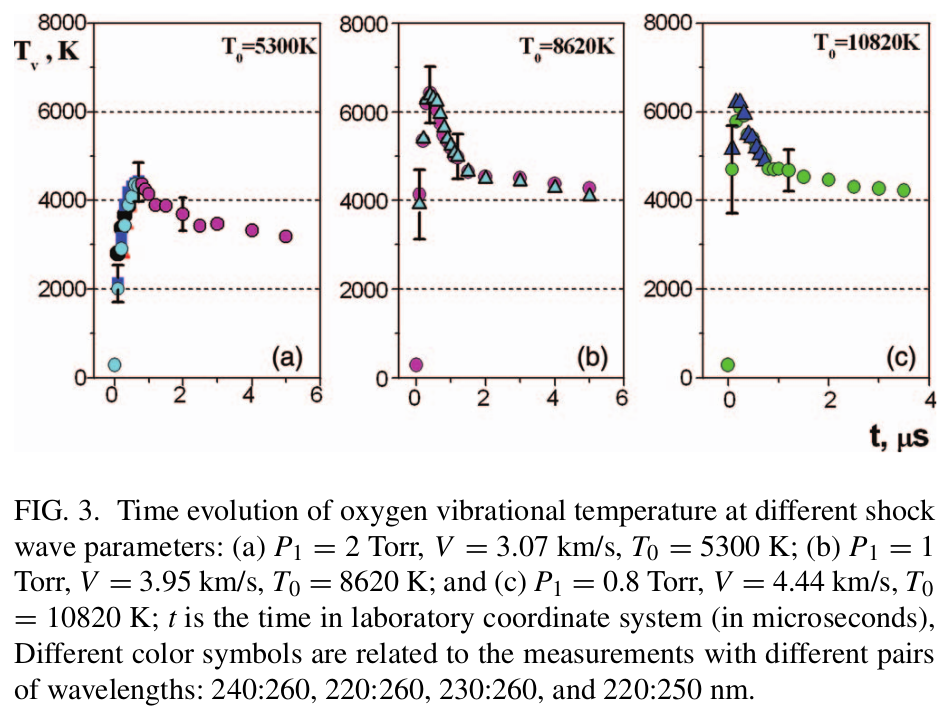
\includegraphics[width=\textwidth]{figures/vibroTemp.png}
\end{figure}
\end{frame}


\section{Oxygen Dissociation}

\begin{frame}
\frametitle{Assumptions}
The determination of the oxygen dissociation rate constant $k_d$ was performed under the following assumptions:
\begin{itemize}
	\item immediately behind the front, only O$_2$-O$_2$ collisions play a role
	in the excitation of oxygen vibrations and dissociation;
	\item for degrees of oxygen dissociation less than 3\%-5\%, observed near
	the front, the role of the newborn atoms as colliding partners in oxygen
	dissociation is negligible;
	\item recombination effects were also not taken into account.
\end{itemize}
\end{frame}

\begin{frame}
\frametitle{Equilibrium Rate Constants}
The thermal equilibrium dissociation rate constant of oxygen
$k_d^0\left(\text{O}_2-\text{O}_2\right)$ was obtained for two ranges of
temperature:
\begin{itemize}
	\item for $T_t<$ 6000 K
	\begin{equation*}
	k_d^0=AT_t^n\left(1-e^{-\Theta_v/T_t}\right)e^{-T_a/T_t}\quad\left[\text{cm}^3\text{mol}^{-1}\text{s}^{-1}\right]
	\end{equation*}
	where $A=2\times10^{15}$, $n=0.3$, $\Theta_v$ is the characteristic vibrational temperature of O$_2$ and $T_a=59380$ K;
	\item for 6000 K $<T_t<$ 11000 K
	\begin{equation*}
	k_d^0=AT_t^ne^{-T_a/T_t}\quad\left[\text{cm}^3\text{mol}^{-1}\text{s}^{-1}\right]
	\end{equation*}
	where $A=3.87\times10^{27}$, $n=-3.1$ and $T_a=59380$ K;
\end{itemize}

In all calculations the oxygen dissociation rate constant for collisions with
atoms O will be given by
\begin{equation*}
k_d^0\left(\text{O}_2-\text{O}\right)=3.5\times k_d^0\left(\text{O}_2-\text{O}_2\right)
\end{equation*}
\end{frame}

\begin{frame}
\frametitle{Thermal Nonequilibrium Dissociation}
For the description of the thermal non-equilibrium dissociation, the well known
CVDV-model of dissociation and vibrational relaxation coupling is used. The
dissociation rate constant is represented usually in the form
\begin{equation*}
k_d\left(T_t,T_v\right)=k_d^0\left(T_t\right)\times Z\left(T_t,T_v\right)
\end{equation*}
where $Z\left(T_t,T_v\right)$ is the coupling factor.

In the study an empirical model for simulation of high temperature ($T_t>$ 6000
K) non-equilibrium processes behind the shock front is proposed with the
following expression for the coupling factor:
\begin{equation*}
Z\left(T_t,T_v\right)=\text{exp}\left[-\alpha\left(1-\frac{T_v}{T_t}\right)\right]
\end{equation*}
\end{frame}

\begin{frame}
The parameter $\alpha$ depends on the temperature $T_t$ and therefore using a
constant value for $\alpha$ is a rough approximation. In light of this, the
temperature dependence for $\alpha$ was estimated in such a way that described
the temperature profiles for all high-temperature regimes accurately:
\begin{equation*}
\alpha=A_1+A_2T_t+A_3T_t^2+A_4T_t^3
\end{equation*}
where $A_1=817.07$, $A_2=-0.243$, $A_3=2.42\times10^{-5}$ and $A_4=-8.05\times10^{-10}$.
\newline\newline
It was assumed that the average vibrational energy $E$, lost by a single act of dissociation, is a constant value
\begin{equation*}
E=0.45\times D_0
\end{equation*}
where $D_0$ is the dissociation energy of a molecule.
\end{frame}


\section{Vibrational Relaxation Time}

%\begin{frame}
%The vibrational relaxation time for diatomic molecules is determined, according
%to Ref. '\textit{L. Landau and E. Teller, Phys. Z. Sowjetunion 10, 34 (1936)}',
%by the following formula:
%\begin{equation*}
%p\tau=\frac{kT_t}{\sigma_0\sqrt{\frac{8RT_t}{\pi \mu}}pP_{10}\left(1-e^{-\Theta_v/T_t}\right)}
%\end{equation*}
%Here $\sigma_0$ is the gas-kinetic effective cross-section of molecule
%collisions with particles of the medium, $P_{10}$ is the probability of molecule
%deactivation from the first vibrational level,
%$P_{10}\propto\text{exp}(T^{1/3})$, and $\mu$ is the reduced molecular weight of
%the colliding particles.
%\end{frame}

\begin{frame}
The vibrational relaxation time for a mixture is given by
\begin{equation} \label{eq:tau_vt}
\tau_s=\frac{\sum\limits_{r\neq e}X_r}{\sum\limits_{r\neq e}X_r/\tau_{sr}}
\end{equation}
where the interspecies relaxation time, $\tau_{sr}$, is expressed as the sum
of Millikan and White contribution, $\tau_{sr}^{\scalebox{0.5}{\textit{MW}}}$,
and Park one, $\tau_{sr}^{\scalebox{0.5}{\textit{P}}}$, as follows
\begin{equation} \label{eq:tau_sr}
\tau_{sr}=\tau_{sr}^{\scalebox{0.5}{\textit{MW}}}+\tau_{sr}^{\scalebox{0.5}{\textit{P}}}
\end{equation}
\end{frame}

\begin{frame}
The first correlation is expressed as
\begin{equation} \label{eq:tau_MW}
\tau_{sr}^{\scalebox{0.5}{\textit{MW}}}=\frac{101325}{p}
e^{\left[A_{sr}\left(T_{tr}^{-1/3}-B_{sr}\right)-18.42\right]}
\end{equation}
where
\begin{equation} \label{eq:MWcoeff}
\begin{split}
A_{sr}&=1.16\times 10^{-3}\mu_{sr}^{1/2}\left(\Theta_v^s\right)^{4/3}
\\ B_{sr}&=0.015\mu_{sr}^{1/4}
\end{split}
\end{equation}
and $\mu_{sr}$, the reduced molecular weight of the colliding species $s$ and
$r$, is given by
\begin{equation} \label{eq:reducedM}
\mu_{sr}=\frac{M_sM_r}{M_s+M_r}
\end{equation}
The values for $A_{sr}$ and $B_{sr}$ can be calculated using the previous
generic expressions or using tabulated data from.
\end{frame}

\begin{frame}
Park's correction is given by
\begin{equation} \label{eq:tau_P}
\tau_{sr}^{\scalebox{0.5}{\textit{P}}}=\frac{1}{\sigma_v\bar{c}_sn_{sr}}
\end{equation}
where $\bar{c}_s$, the average molecular velocity of molecule $s$, is
expressed by
\begin{equation} \label{eq:molVel}
\bar{c}_s=\sqrt{\frac{8\Re T_{tr}}{\pi M_s}}
\end{equation}
and $n_{sr}$ is the number density of the colliding pair $\left(s,r\right)$.
The effective cross section for vibrational relaxation, $\sigma_v$, is given
by
\begin{equation} \label{eq:effCrossSection}
\sigma_v=\sigma_v^*\left(\frac{50000}{T_{tr}}\right)^2
\end{equation}
where $\sigma_v^*$ is set to 3.0$\times10^{-21}$ m$^2$ as proposed by Park.
\end{frame}

\begin{frame}
The previous formulation represents the vibrational relaxation time of molecules
at temperatures for which the main statements of the Landau-Teller theory are
valid, in particular, the assumption of adiabaticity of collisions, the
applicability of the harmonic oscillator model and the influence of only the
repulsive part of the interaction potential on the relaxation process.
\end{frame}

%\begin{frame}
%The previous formulation represents the vibrational relaxation time of molecules
%at temperatures for which the main statements of the Landau-Teller theory are
%valid, in particular, the assumption of adiabaticity of collisions, the
%applicability of the harmonic oscillator model and the influence of only the
%repulsive part of the interaction potential on the relaxation process.
%\newline\newline
%Based on available experimental data expression for O$_2$-O$_2$ and O$_2$-O collisions become
%\begin{equation*}
%p\tau=\frac{\alpha e^{\beta T_t^{-1/3}}T_t^{1/2}}{1-e^{-\Theta_v/T_t}}\qquad [\text{atm s}]
%\end{equation*}
%where the constants are listed in table.
%\begin{table}[ht]
%	\centering
%	\renewcommand{\arraystretch}{1.2}
%	\begin{tabular}{ *{4}{c} }
%		\noalign{\hrule height 1pt}
%		\textbf{Collision} & $\boldsymbol{\alpha}$ & $\boldsymbol{\beta}$
%		& $\boldsymbol{\Theta_v}$ \\
%		\hline
%		O$_2$-O$_2$ & 8.8e-14 & 172.7 & 2238 \\ 
%		O$_2$-O & 1.5e-12 & 86.4 & 2238 \\
%		\noalign{\hrule height 1pt}		
%	\end{tabular}
%	\label{tab:const}
%\end{table}
%\end{frame}

\begin{frame}
All of the data on oxygen vibrational relaxation time discussed here are
presented in the next figure. At temperatures $T_t<6000$ K the experimental data
are shown to be well described by Millikan-White approximation (curve 1).
However, at higher temperatures the quantities log$_{10}(p\tau)$ deviate from
this dependence. Accounting for pre-exponential factors, the Landau-Teller theory
gives a deviation from the linear relationship (curve 2). The experimental data
of the present work at $T_t>6000$ K are presented by magenta symbols and curve
3. The temperature dependence of this curve is following:
\begin{equation*}
\text{log}_{10}\left(p\tau_{\scalebox{0.5}{O$_2$-O$_2$}}\right)=a+bx+cx^2+dx^3
\end{equation*}
with $x=T^{-1/3}$ and $a=1.11$, $b=-407.1$, $c=6600.9$, and $d=-31307.9$.
\end{frame}

\begin{frame}
\begin{figure}[ht]
\centering
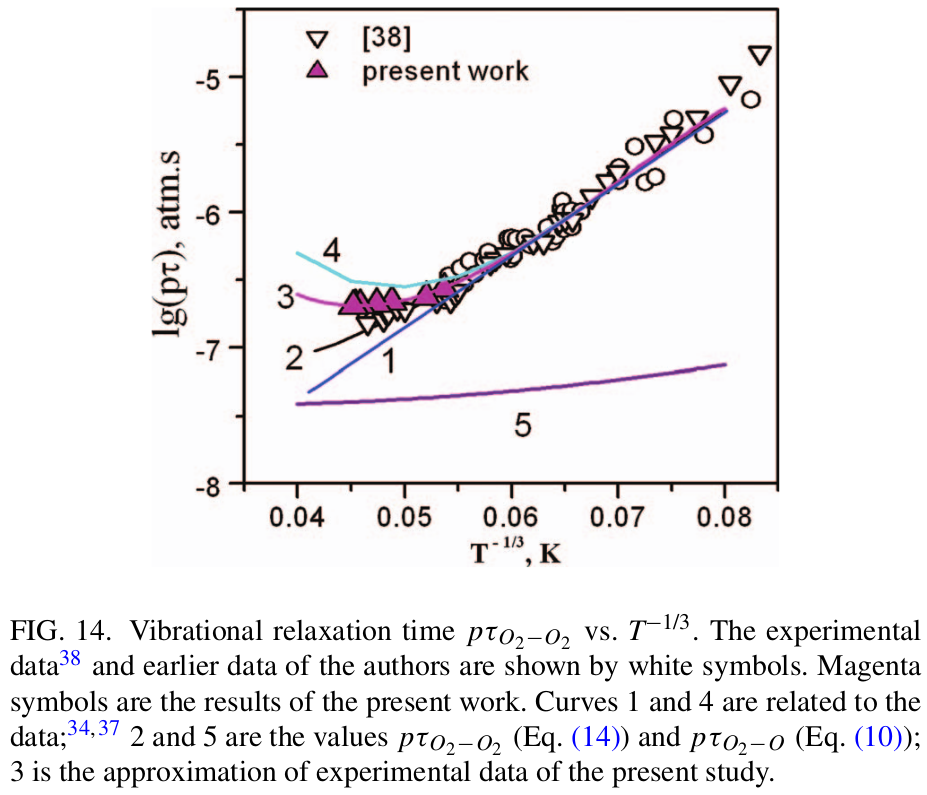
\includegraphics[width=\textwidth]{figures/relaxTime.png}
\end{figure}
\end{frame}


\section{Downstream Gas Parameters}

\begin{frame}
\frametitle{Solving System}
Behind the front of a stationary shock wave the gas flow is governed by the
equations of conservation of the fluxes of mass, momentum, energy, and component
composition:
\begin{align*}
& \rho_1V=\rho_2v_2 \\
& P_1+\rho_1V^2=P_2+\rho_2v_2^2 \\
& h_1(T_{t_1},T_{v_1})+\frac{1}{2}V^2=h_2(T_{t_2},T_{v_2})
+\frac{1}{2}v_2^2 \\
& P=\rho RT_t
\end{align*}
where $V$ is the shock velocity and $v_2$ is the gas flow velocity relative to
the shock front; $T_t$, $P$ and $\rho$ are the gas translational temperature,
pressure, and density; $h$ is the enthalpy of oxygen molecules and atoms. The
state of the gas is denoted by the subscript 1 ahead of the shock front, and 2
behind the front.
\end{frame}

\begin{frame}
The downstream enthalpy $h_2$ in the right side of the equation of energy
conservation for the dissociating gas behind the shock front was represented in
the following form:
\begin{equation*}
h_2(T_{t_2},T_{v_2})=\frac{7}{2}RT_{t_2}+e_{ve}(T_{v_2})
\end{equation*}
Knowing the experimental values of $T_{v_2}$, it's possible to obtain the downstream flow conditions $t=0$ s by solving the previous system with the following iterative method by assuming a pure O$_2$ freestream composition at the inlet section $\left(R=R_u/M_{O_2}\right)$ and knowing the upstream conditions made of $T_{t_1}=T_{v_1}=295$ K, $P_1$ and $V$ (3 different cases).
\end{frame}

\begin{frame}
Guessing the initial value of $\rho_2^{(0)}=1$, the iterative method will be
\begin{align*}
& v_2^{(n)}=\frac{\rho_1V}{\rho_2^{(n)}} \\
& P_2^{(n)}=P_1+\rho_1V^2-\rho_2^{(n)}\left(v_2^{(n)}\right)^2 \\
& h_2^{(n)}=h_1+\frac{1}{2}V^2-\frac{1}{2}\left(v_2^{(n)}\right)^2 \\
& T_{t_2}^{(n)}=\frac{2}{7}\left(\frac{h_2^{(n)}-e_{ve}(T_{v_2})}{R}\right) \\
& \rho_2^{(n+1)}=\frac{P_2^{(n)}}{RT_{t_2}^{(n)}} \\
& until \\
& \text{err}=\Big|\rho_2^{(n+1)}-\rho_2^{(n)}\Big|<\text{tol}
\end{align*}
\end{frame}


\end{document}
